\documentclass{../c-lecture}

\subtitle{Functions}

\begin{document}

\begin{frame}
  \titlepage{}
\end{frame}
\begin{frame}
  \frametitle{Outline}
  \tableofcontents{}
\end{frame}

\section{Introduction}

\begin{frame}
  \frametitle{Introduction}
  \begin{itemize}
    \item Until now, we learned to develop simple algorithms
    \begin{itemize}
      \item Interactions, Mathematics, Decisions, and Loops
    \end{itemize}
    \item Real problems: very complex
    \begin{itemize}
      \item Compressing a file
      \item Calculator
      \item Games, MS Word, Firefox, \ldots
    \end{itemize}
    \item Cannot be developed at once
    \begin{itemize}
      \item Divide the problem into smaller sub-problems
      \item Solve the sub-problems
      \item Put the solutions altogether to get the final solution
    \end{itemize}
    \item \textbf{\color{Melon} Modular} programming
  \end{itemize}
\end{frame}

\begin{frame}
  \frametitle{Modular programming}
  \begin{itemize}
    \item Solving a large and complex problem
    \item Design the overall algorithm
    \item Some portions are <span class="hl-orange">black-box</span>
    \begin{itemize}
      \item We know <span class="hl-green">what</span> each box does
      \item But we don't worry <span class="hl-cyan">how</span>
      \item Later, we think about the black-boxes and develop them
    \end{itemize}
    \item
      Black-boxes are implemented by \textbf{\color{RubineRed} functions}
  \end{itemize}
\end{frame}

\begin{frame}
  \frametitle{Modular programming: Advantages}
  \begin{itemize}
    \item Easy to develop and understand
    \item Reusability
    \begin{itemize}
      \item Something is used frequently
      \begin{itemize}
        \item Mathematic: Square, Power, Sin, \ldots
        \item Programming: Printing, Reading
      \end{itemize}
      \item
        Develop it \textbf{\color{Orange} one time}, use it
        \textbf{\color{LimeGreen} many times}
    \end{itemize}
    \item Multiple developers can work on different parts
    \item Each module can be tested and debugged separately
  \end{itemize}
\end{frame}

\begin{frame}[fragile]
  \frametitle{Functions in C}
  \begin{itemize}
    \item Functions in mathematics
    \begin{itemize}
      \item \mint{c}|z = f(x, y)|
    \end{itemize}
    \item Functions in C
    \begin{itemize}
      \item \textbf{\color{YellowOrange} Queries}: Return a value
      \begin{itemize}
        \item \mint{c}|sin()|, \mint{c}|fabs()|
      \end{itemize}
      \item
        \textbf{\color{LimeGreen} Commands}: do some tasks, do not return
        any value
      \begin{itemize}
        \item \mint{c}|printf_my_info(...)|
      \end{itemize}
    \end{itemize}
  \end{itemize}
\end{frame}

\begin{frame}
  \frametitle{Functions in C}
  Three steps to use functions in C:
  \begin{enumerate}
    \item Function prototype (declaration)
    \begin{itemize}
      \item Introduce the function to compiler
    \end{itemize}
    \item Function definition
    \begin{itemize}
      \item What the function does
    \end{itemize}
    \item Function call
    \begin{itemize}
      \item Use the function
    \end{itemize}
  \end{enumerate}
\end{frame}

\begin{frame}[fragile]
  \frametitle{Function \textbf{prototype}}
  \mint{c}|<output type> <function name>(<input parameter types>);|
  \begin{itemize}
    \item <output type>
    \begin{itemize}
      \item \textmd{\color{Orange} Queries}: int, float, \ldots
      \item \textmd{\color{LimeGreen} Command}: void
    \end{itemize}
    \item
      <function name> is an identifier
    \item <input parameter types>
    \begin{itemize}
      \item <type>, <type>, \ldots
      \begin{itemize}
        \item int, float, \ldots
      \end{itemize}
      \item void
    \end{itemize}
  \end{itemize}
\end{frame}

\begin{frame}[fragile]
  \frametitle{Function \textbf{definition}}
  \begin{minted}[bgcolor=Black]{c}
<output type> <function name>(<input parameters>) {
  <statements>
}
  \end{minted}
  \begin{itemize}
    \item <output type>
    \begin{itemize}
      \item \textmd{\color{Orange} Queries}: int, float, \ldots
      \item \textmd{\color{LimeGreen} Command}: void
    \end{itemize}
    \item
      \textit{\color{LimeGreen} <function name>} is an identifier
    \item \textit{\color{Cyan} <input parameter>}
    \begin{itemize}
      \item
        <type> <identifier>, <type> <identifier>, \ldots
      \begin{itemize}
        \item int in, float f, \ldots
      \end{itemize}
      \item void
    \end{itemize}
  \end{itemize}
\end{frame}

\begin{frame}
  \begin{itemize}
    \item Function definition should be out of other functions
    \begin{itemize}
      \item Function in function is not allowed
    \end{itemize}
  \end{itemize}
\end{frame}

\begin{frame}
  \frametitle{Function call}
  \begin{itemize}
    \item Command function
    \textit{\color{LimeGreen} <function name>(inputs)}
    \item Query function
    \textit{\color{LimeGreen} <variable> = <function name>(inputs)}
    \item Inputs should match by function definition
    \item Functions are called by another function
    \begin{itemize}
      \item Function call comes inside in a function
    \end{itemize}
  \end{itemize}
\end{frame}

\begin{frame}[fragile]
  \frametitle{Example}
  \begin{minted}[bgcolor=Black]{c}
/* Function declaration */
void my_info(void);

int main(void){
  printf("This is my info");
  my_info(); /* Function call */
  printf("=============");
  return 0;
}

/* Function definition */
void my_info(void){
  printf("Student name is Parham Alvani\n");
  printf("Student number: 9231058\n");
}
  \end{minted}
\end{frame}

\begin{frame}[fragile]
  \frametitle{Example}
  \begin{minted}[bgcolor=Black]{c}
/* Function definition */
void my_info(void) {
  printf("Student name is Parham Alvani\n");
  printf("Student number: 9231058\n");
}

int main(void) {
  printf("This is my info");
  my_info(); /* Function call */
  printf("=============");
  return 0;
}
  \end{minted}
\end{frame}

\begin{frame}
  \frametitle{Function Declaration?!!!!}
  \begin{itemize}
    \item Is function declaration needed?
    \item Is there any useful application of function declaration?
    \item \textbf{\color{Orange} Yes!}
    \item Libraries are implemented using it
    \begin{itemize}
      \item .h files contains the function declarations
      \item and also other definitions
      \item .so, .a, .dll, \ldots are the compiled function definitions
    \end{itemize}
  \end{itemize}
\end{frame}

\section{Passing input parameters}

\begin{frame}[fragile]
  \frametitle{Input Parameters}
  \begin{itemize}
    \item Inputs of function
    \begin{itemize}
      \item No input: \textit{\color{YellowOrange} void}
      \item One or multiple inputs
    \end{itemize}
    \item Each input should have a type
    \item Input parameters are split by ``,''
    \begin{minted}[bgcolor=Black]{c}
void f(void)
void f(int a)
void f(int a, float b)
void f(int a, b) // compile error
    \end{minted}
  \end{itemize}
\end{frame}

\begin{frame}[fragile]
  \begin{minted}[bgcolor=Black]{c}
#include <stdio.h>

void print_sub(double a, double b) {
  double res;
  res = a - b;
  printf("Sub of %lf and %lf is %lf\n", a, b, res);
}

int main(void) {
  double d1 = 10, d2 = 20;
  print_sub(56.0, 6.0);
  print_sub(d1, d2);
  print_sub(d1, d2 + d2);
  return 0;
}
  \end{minted}
\end{frame}

\begin{frame}
  \frametitle{How Does Function Call Work?}
  \begin{itemize}
    \item
      Function call is implemented by \textit{\color{YellowOrange} ``stack''}
    \item
      Stack is a \textit{\color{LimeGreen} logical} part of the main memory
    \item Variables of function and its input variables are in stack
    \item When a function calls
    \begin{itemize}
      \item Its variables including the inputs are allocated in stack
      \item
        The value of input parameters from caller function is pushed to stack of
        called function
      \begin{itemize}
        \item
          They are \textbf{\color{Cyan} copied} in to the variables of
          function
      \end{itemize}
    \end{itemize}
    \item When function finished, its stack is freed
  \end{itemize}
\end{frame}

\begin{frame}[fragile]
  \frametitle{print_sub: What happen?}
  \mint{c}|print_sub(56.0, 6.0);|
  \begin{itemize}
    \item 56.0 is copied the memory location \textbf{\color{LimeGreen} a}
    \item 6.0 is copied to memory location \textbf{\color{Orange} b}
  \end{itemize}
  \begin{minted}[bgcolor=Black]{c}
double a = 56.0;
double b = 6.0;
double res;
res = a - b;
  \end{minted}
\end{frame}

\begin{frame}[fragile]
  \frametitle{print_sub: What happen?}
  \mint{c}|print_sub(d1, d2);|
  \begin{itemize}
    \item
      value of d1 is copied the memory location
      \textit{\color{LimeGreen} a}
    \item
      value of d2 is copied to memory location
      \textit{\color{YellowOrange} b}
  \end{itemize}
  \begin{minted}[bgcolor=Black]{c}
double a = 10.1;
double b = 6.0;
double res;
res = a - b;
  \end{minted}
  \textbf{\color{RubineRed} Call by Value}
\end{frame}

\begin{frame}
  \frametitle{Call by value}
  \begin{itemize}
    \item In call by value mechanism
    \begin{itemize}
      \item
        The values are \textit{\color{Orange} copied} to the function
    \end{itemize}
    \item If we change values in the function
    \begin{itemize}
      \item The copied version is changed
      \item
        The original value does \textit{\color{RubineRed} not} affected
    \end{itemize}
    \item
      Call by value inputs \textit{\color{RubineRed} cannot} be used to
      produce output
  \end{itemize}
\end{frame}

\begin{frame}
  \begin{figure}
    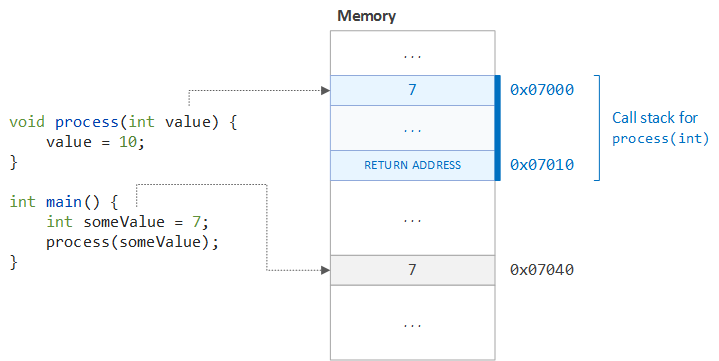
\includegraphics[width=\textwidth]{./img/pass-by-value.png}
  \end{figure}
\end{frame}

\begin{frame}
  \frametitle{Call by Reference}
  \begin{itemize}
    \item
      The local parameters are
      \textbf{\color{Orange} references} to the storage locations of
      the original arguments passed in.
    \item
      Changes to these variables in the function
      \textbf{\color{LimeGreen} will affect} the originals
    \item
      \textit{\color{Cyan} No copy is made}, so overhead of copying
      (time, storage) is saved
  \end{itemize}
\end{frame}

\begin{frame}[fragile]
  \frametitle{add function (wrong version)}
  \begin{minted}[bgcolor=Black]{c}
void add(double a, double b, double res){
  res = a + b;
  return;
}

int main(void){
  double d1 = 10.1, d2 = 20.2;
  double result = 0;
  add(56.0, 6.7, result);
  printf("result = %lf\n", result);
  add(d1, d2, result);
  printf("result = %lf\n", result);
}
  \end{minted}
\end{frame}

\section{Producing output}

\begin{frame}
  \frametitle{Producing output}
  \begin{itemize}
    \item What we have seen are the “Command”
    \item Query functions
    \begin{itemize}
      \item Produce output
      \item
        Output <span class="hl-red">cannot</span> be produced by the “call by
        value” parameters

    \end{itemize}
    \item To produce an output
    \begin{itemize}
      \item Declare output type
      \item Generate the output by <span class="hl-orange">return</span>
    \end{itemize}
  \end{itemize}
\end{frame}

\begin{frame}{fragile}
  \frametitle{The return command}
  \begin{itemize}
    \item To generate a result by a function
    \mint{c}|return <value>;|
    \item Only one value can be returned
    \item <span class="hl-green">return</span> finishes running the function
    \item Function can have multiple return
    \begin{itemize}
      \item Only one of them runs each time
    \end{itemize}
    \item The type of the returned value = the result type
    \begin{itemize}
      \item Otherwise, cast
    \end{itemize}
  \end{itemize}
\end{frame}

\begin{frame}
  \frametitle{Exmaple: my_fabs (Version 1)}
  \begin{minted}[bgcolor=Black]{c}
double my_fabs(double x){
  double res;
  if(x >= 0)
    res = x;
  else
    res = -1 * x;
  return res;
}

void main(void){
  double d = -10;
  double b;
  b = my_fabs(d);
  printf("%lf\n", b);
  printf("%lf\n", my_fabs(-2 * b));
}
  \end{minted}
\end{frame}

\begin{frame}[fragile]
  \frametitle{Exmaple: my_fabs (Version 2)}
  \begin{minted}[bgcolor=Black]{c}
double my_fabs(double x){
  if(x >= 0)
    return x;
  return (-1 * x);
}

void main(void){
  double d = -10;
  double b;
  b = my_fabs(d);
  printf("b = %lf\n", b);
  b = my_fabs(-2 * d);
  printf("b = %lf\n", b);
}
  \end{minted}
\end{frame}

\begin{frame}[fragile]
  \frametitle{Output of functions}
  \begin{itemize}
    \item
      A function can produce
      <span class="hl-orange">at most one</span> output

    \item Output of functions can be dropped
  \end{itemize}
  \begin{minted}[bgcolor=Black]{c}
double f;
sin(f); // we drop the output of sin
gcd(10, 20); // we drop the output of gcd
  \end{minted}
\end{frame}

\begin{frame}[fragile]
  \frametitle{Casting in functions}
  \begin{itemize}
    \item Cast for input
    \begin{itemize}
      \item
        Prototype: <span class="hl-orange">void f(int a, double b);</span>

      \item Call: <span class="hl-green">f(10.1, 20.2);</span>
    \end{itemize}
    \item Cast for output
    \begin{itemize}
      \item Prototype: <span class="hl-orange">int f(int a);</span>
      \item Call: <span class="hl-green">double d = f(10);</span>
      \item In return: <span class="hl-cyan">return 10.20</span>
    \end{itemize}
  \end{itemize}
\end{frame}

\begin{frame}[fragile]
  \frametitle{Be careful: empty input/output type}
  \begin{itemize}
    \item
      If output or input type is not specified:
      \textbf{\color{Orange} int}
    \begin{itemize}
      \item Casting may not work
    \end{itemize}
  \end{itemize}
  \begin{minted}[bgcolor=Black]{c}
f1(a){
  printf("a = %d\n", a); return a / 2;
}

f2(int a){
  printf("a = %d\n", a); return a / 2;
}

f3(float a){
    printf("a = %f\n", a);  return a / 2;
}

int main(){
  printf("%d\n", f1(10.5));
  printf("%d\n", f2(10.5));
  printf("%d\n", f3(10.5));
  return 0;
}
  \end{minted}
\end{frame}

\begin{frame}
  \frametitle{Inline Functions \& Macro}
  \begin{itemize}
    \item Function call using stack has its overhead
    \begin{itemize}
      \item 2 approaches to reduce the overhead
    \end{itemize}
    \item <span class="hl-orange">inline</span> function
    \begin{itemize}
      \item To ask from compiler to compile it as inline, but no guarantee
      \item
        <span class="hl-green">GCC</span> and
        <span class="hl-green">Clang</span> don't support
        <span class="hl-orange">inline</span> functions

      <pre><code class="hljs lang-c">
inline int f(float x)
      </code></pre>
    \end{itemize}
    \item Macros
    \begin{minted}[bgcolor=Black]{c}
#define PRINT_INT(X) printf("%d\n", X)
    \end{minted}
  \end{itemize}
\end{frame}

\begin{frame}
  \frametitle{Example: GCD}
  \begin{minted}[bgcolor=Black]{c}
#define PRINT_INT(x) printf("%d\n",x); \
                      printf("===================\n");

inline int gcd(int a, int b){ /* return gcd of a and b */
  int temp;
  while(b != 0){
    temp = a % b;
    a = b;
    b = temp;
  }
  return a;
}

void main(void){
  int i = 20, j = 35, g;

  g = gcd(i, j);
  printf("GCD of %d and %d = ", i , j);
  PRINT_INT(g);

  g = gcd(j, i);
  printf("GCD of %d and %d = ", j , i);
  PRINT_INT(g);
}
  \end{minted}
\end{frame}

\section{Scope of variables}

\begin{frame}
  \frametitle{Scope of Variables}
  \begin{itemize}
    \item Variables
    \begin{itemize}
      \item Are declared in the start of functions
      \item
        Are used any where in the function
        <span class="hl-orange">after declaration</span>

      \item Cannot be used outside of function
      \item Cannot be used in other functions
    \end{itemize}
    \item <span class="hl-orange">Scope</span> of variable
    \begin{itemize}
      \item A range of code that the variable can be used
    \end{itemize}
    \item Variable cannot not be used outside of its scope
    \begin{itemize}
      \item Compile error
    \end{itemize}
  \end{itemize}
\end{frame}

\begin{frame}
  \frametitle{Scopes and Blocks}
  \begin{itemize}
    \item Scopes are determined by Blocks
    \begin{itemize}
      \item Start with { and finished by }
      \item
        Example: statements of a function, statement of a if or while, ...

    \end{itemize}
    \item Variables
    \begin{itemize}
      \item <span class="hl-orange">Can be</span> declared in a block
      \item <span class="hl-green">Can be</span> used in the declared block
      \item
        <span class="hl-cyan">Cannot be</span> used outside the declared block

    \end{itemize}
    \item The declared block is the scope of the variable
  \end{itemize}
\end{frame}

\begin{frame}[fragile]
  \frametitle{Variables in Blocks}
  \begin{minted}[bgcolor=Black]{c}
#include <stdio.h>

int main(void){
  int i;
  for(i = 1; i <= 10; i++){
    int number;
    printf("Enter %d-th number: ", i);
    scanf("%d", &number);

    if((number % 2) == 0)
        printf("Your number is even\n");
     else
         printf("Your number is odd\n");
  }
  /* compile error
   printf("The last number is %d\n", number); */
  return 0;
}
  \end{minted}
\end{frame}

\begin{frame}
  \frametitle{Nested Scopes/Blocks}
  \begin{itemize}
    \item Scopes can be nested
    \begin{itemize}
      \item Example: Nested if, nested for, ...
    \end{itemize}
  \end{itemize}
  \begin{minted}[bgcolor=Black]{c}
void main(){ // block 1
  int i;
  { // block 2
    int j;
    { // block 3
       int k;
    }
    int m;
  }
}
  \end{minted}
\end{frame}

\begin{frame}
  \frametitle{Variables in Nested Blocks}
  \begin{itemize}
    \item All variables from outer block can be used inner blocks
    \begin{itemize}
      \item Scope of inner block contains the outer block
    \end{itemize}
    \item
      Variables in inner block <span class="hl-red">cannot</span> be used in
      outer block

    \begin{itemize}
      \item
        Scope of the outer block
        <span class="hl-red">does not</span> contains the inner block

    \end{itemize}
  \end{itemize}
\end{frame}

\begin{frame}[fragile]
  \frametitle{Variables in Nested Blocks: Example}
  \begin{minted}[bgcolor=Black]{c}
int k;

for(int i = 0; i <; 10; i++){
  /* block 1 */
  if(i > 5){
    /* block 2 */
    int j = i;
    ...
  }

  while(k > 10){
    /* block 3 */
    int l = i;
    /* int m = j; compile error */
    ...
  }

  /* k = l; compile error */
}
  \end{minted}
\end{frame}

\begin{frame}
  \frametitle{Variables in Nested Blocks: Example}
  \begin{itemize}
    \item
      If a variable in inner block has the same identifier of a variable in
      outer block

    \begin{itemize}
      \item
        The inner variable <span class="hl-orange">hides</span> the outer
        variable

      \item
        Changing inner variables
        <span class="hl-green">does not</span> change outer variable

    \end{itemize}
  \end{itemize}
  <p class="hl-red" style="font-size: 120px">Do Not Use It</p>
\end{frame}

\begin{frame}
  \frametitle{Local Variables}
  \begin{itemize}
    \item
      All variables defined in a function are the
      <span class="hl-orange">local variable</span> of the function

    \item
      Can <span class="hl-green">ONLY</span> be used in the function, not other
      functions

  \end{itemize}
  \begin{minted}[bgcolor=Black]{c}
void func(void){
  /* These are local variables */
  int i, j;
  float f;
}

int main(void){
  i = 10; /* compile error, why? */
  f = 0; /* compile error, why? */
}
  \end{minted}
\end{frame}

\begin{frame}[fragile]
  \frametitle{Global/External Variables}
  \begin{itemize}
    \item Global variables are defined outside of all functions
    \item
      Global variables are <span class="hl-orange">initialized</span> to
      <span class="hl-cyan">zero</span>

    \item
      Global variables are available to all
      <span class="hl-green">subsequent</span> functions

  \end{itemize}
  \begin{minted}[bgcolor=Black]{c}
void f(){
   i = 0; // compile error
}
int i;
void g(){
   int j = i; // g can use i
}
  \end{minted}
\end{frame}

\begin{frame}[fragile]
  \frametitle{Global/External Variables: Example}
  \begin{minted}[bgcolor=Black]{c}
int i, j;
float f;

void func(void){
  printf("i = %d \n", i);
  printf("f = %f \n", f);
  i = 20;
}

void f1(){
  printf("%d", i);
}

int main(void){
  f = 1000;
  func();
  f1();
  return 0;
}
  \end{minted}
\end{frame}

\begin{frame}[fragile]
  \frametitle{Parameter Passing by Global Variables: my_fabs (V.3)}
  \begin{minted}[bgcolor=Black]{c}
double x;

void my_fabs(void){
  x = (x > 0) ? x : -1 * x;
}

void main(void){
  double b, d = -10;
  x = d;
  my_fabs();
  b = x;
  printf("b = %f\n", b);
}
  \end{minted}
\end{frame}
\begin{frame}
  \begin{itemize}
    \item
      <span class="hl-red">Don’t</span> use this method. Parameters should be
      passed by input parameter list.

    \item
      Global variable are used to define (large) variables that are used in
      many functions

  \end{itemize}
\end{frame}

\section{Storage Class of variables}

\begin{frame}
  \begin{itemize}
    \item Storage class
    \begin{itemize}
      \item How memory is allocated for the variable
      \item Until when the variable exists
      \item How it is initialized
    \end{itemize}
    \item Storage classes in C
    \begin{itemize}
      \item Automatic
      \item External
      \item Static
      \item Register
    \end{itemize}
  \end{itemize}
\end{frame}

\begin{frame}
  \frametitle{Storage Classes: Automatic}
  \begin{itemize}
    \item All local variables are automatic by default
    \begin{itemize}
      \item Input parameters of a function
      \item Variables defined inside a function/block
      \item
        Keyword <span class="hl-orange">auto</span> is optional before them
    \end{itemize}
    \item
      Generated at the
      <span class="hl-green">start of each run of the block</span>

    \item
      Destroyed at the
      <span class="hl-cyan">end of each run of the block</span>

    \item Are not initialized
  \end{itemize}
\end{frame}

\begin{frame}
  \begin{frame}
    \frametitle{Storage Classes: External}
    \begin{itemize}
      \item All global variables are external by default
      \begin{itemize}
        \item Are initialized by 0
        \item Are generated when program starts
        \item Are destroyed when program finishes
      \end{itemize}
      \item Usage of keyword <span class="hl-orange">extern</span>
      \begin{itemize}
        \item To use global variables in other files
        \item To use global variables before definition
        \item To emphasize that variable is global
        \begin{itemize}
          \item This usage is optional
        \end{itemize}
      \end{itemize}
    \end{itemize}
  \end{frame}
  \begin{frame}
    \begin{itemize}
      \item We only declare <code>var</code> and later define it.
    \end{itemize}
    <pre><code class="lang-c">
#include <stdio.h>;

extern int var;

int main(void)
{
  printf("%d\n", var);
  return 0;
}

int var = 20;
    </code></pre>
    \begin{itemize}
      \item We declare and define <code>var</code>. (optional usage)
    \end{itemize}
    <pre><code class="lang-c">
#include <stdio.h>

extern int var = 10;

int main(void)
{
  printf("%d\n", var);
  return 0;
}
    </code></pre>
  \end{frame}
\end{frame}
\begin{frame}
  \frametitle{Storage Classes: Static}
  \begin{itemize}
    \item Keyword <span class="hl-orange">static</span> comes before them
    \item For <span class="hl-yellow">local</span> variables:
    \begin{itemize}
      \item
        Generated in
        <span class="hl-green">the first run of the block</span>

      \item Destroyed <span class="hl-cyan">when program finishes</span>
      \item Initialized
      \begin{itemize}
        \item If no value &rarr; initialized by 0
        \item Only initialized in the first run of the block
      \end{itemize}
    \end{itemize}
  \end{itemize}
\end{frame}
\begin{frame}
  \frametitle{Storage Classes: Static (Cont.)}
  \begin{itemize}
    \item Keyword <span class="hl-orange">static</span> comes before them
    \item For <span class="hl-yellow">global</span> variables:
    \begin{itemize}
      \item Generated <span class="hl-green">when program starts</span>
      \item Destroyed <span class="hl-cyan">when program finishes</span>
      \item Initialized
      \begin{itemize}
        \item If no value &rarr; initialized by 0
      \end{itemize}
      \item Is not accessible for other files
    \end{itemize}
  \end{itemize}
\end{frame}
\begin{frame}
  \frametitle{Storage Classes: Register}
  \begin{itemize}
    \item Keyword <span class="hl-orange">register</span> comes before them
    \item Can be used for local variables
    \item Compiler tries to allocated the variable in registers of CPU
    \begin{itemize}
      \item But does <span class="hl-red">not</span> guaranteed
      \item Registers are very fast and small memories
    \end{itemize}
    \item Improve performance
  \end{itemize}
\end{frame}
\begin{frame}
  \frametitle{Storage Classes, Auto: Examples}
  <pre><code class="hljs lang-c">
void f(int i, double d){
  int i2;
  auto int i3;
  double d2;
  auto double d3;
}
  </code></pre>
  <p>All variables (i, d, i2, i3, d2, d3) are auto variables</p>
\end{frame}
\begin{frame}
  \frametitle{Storage Classes, Extern: Examples}
  <pre><code class="hljs lang-c">
int i = 10, j = 20;

void print(void){
  printf("i = %d, j = %d\n", i, j);
}

int main(void){
  extern int i; // i refers the global i
  int j;
  print();
  i = 1000;
  j = 2000;
  print();
  return 0;
}
  </code></pre>
\end{frame}

\begin{frame}[fragile]
  \frametitle{Storage Classes: Examples}
  <pre><code class="hljs lang-c">
int i;

void func(void){
  int j;
  printf("i = %d \n", i);
  printf("j = %d \n", j);
  i = 20;
}

int main(void){
  func();
  func();
  i = 30;
  func();
  return 0;
}
  </code></pre>
\end{frame}

\begin{frame}[fragile]
  \frametitle{Storage Classes, Static: Examples}
  <pre><code class="hljs lang-c">
void func(void){
  int j;
  static int i;
  printf("i = %d \n", i);
  printf("j = %d \n", j);
  i = 20;
}
int main(void){
  func();
  func();
  /* i = 30; compile error, why? */
  func();
  return 0;
}
  </code></pre>
\end{frame}

\begin{frame}
  \frametitle{Storage Classes, Register: Examples}
  <pre><code class="hljs lang-c">
register int i;
for(i = 0; i <; 100; i++)
  </code></pre>
\end{frame}

\begin{frame}
  \frametitle{Be careful: loop \& automatic variables}
  \begin{itemize}
    \item According to standard:
    \begin{block}{}
      For such an object that does not have a variable length array type, its
      lifetime extends from entry into the block with which it is associated
      until execution of that block ends in any way.
    \end{block}
    \item Variable is \textit{\color{Yellow} defined in a block of a loop}
    \item
      The variable retains its value between iterations of the loop if it is
      \textbf{\color{RubineRed} NOT} variable length array
    \item
      The variable does \textbf{\color{RubineRed} NOT} retain its value between
      iterations of the loop if it is a variable length array
  \end{itemize}
\end{frame}

\begin{frame}
  \begin{frame}
    \frametitle{loop &amp; automatic variables}
    <pre><code class="hljs lang-c">
int main(){
  int i;
  for(i = 0; i <; 5; i++) {
    int j;
    if(i) { // when i != 0 update j
      printf("&amp;j = %p, j = %d\n", &amp;j, j);
      j++;
    } else { // when i == 0 set j to 0
      j = i;
    }
  }
}
    </code></pre>
  \end{frame}
  \begin{frame}
    <pre><code>
&j = 0x7ffeed9f3964, j = 0
&j = 0x7ffeed9f3964, j = 1
&j = 0x7ffeed9f3964, j = 2
&j = 0x7ffeed9f3964, j = 3
    </code></pre>
  \end{frame}
\end{frame}

\begin{frame}
  \begin{frame}
    \frametitle{loop &amp; automatic variables}
    <pre><code class="hljs lang-c">
int main(){
  int i;
  for(i = 0; i <; 5; i++) {
    int j[5 * i + 1];
    if(i) {
      printf("&amp;j[0] = %p, j[0] = %d\n", (&amp;j[0]), j[0]);
      j[0]++;
    } else {
      j[0] = i;
    }
  }
}
    </code></pre>
  \end{frame}
  \begin{frame}
    <pre><code>
&amp;j[0] = 0x7ffee735b910, j[0] = -415909520
&amp;j[0] = 0x7ffee735b900, j[0] = -415909520
&amp;j[0] = 0x7ffee735b8f0, j[0] = -415909520
&amp;j[0] = 0x7ffee735b8d0, j[0] = -415909872
    </code></pre>
  \end{frame}
\end{frame}

\begin{frame}[fragile]
  \frametitle{loop \& automatic variables}
  \begin{minted}[bgcolor=Black]{c}
int main(){
  int i;
  for(i = 0; i <; 5; i++) {
    int j[5 * 3 + 1];
    if(i) {
      printf("&j[0] = %p, j[0] = %d\n", (&j[0]), j[0]);
      j[0]++;
    } else {
      j[0] = i;
    }
  }
}
  \end{minted}
\end{frame}

\begin{frame}[fragile]
  \begin{minted}[bgcolor=Black]{output}
&j[0] = 0x7ffee2a4d920, j[0] = 0
&j[0] = 0x7ffee2a4d920, j[0] = 1
&j[0] = 0x7ffee2a4d920, j[0] = 2
&j[0] = 0x7ffee2a4d920, j[0] = 3
  \end{minted}
\end{frame}

\section{Function usage example}

\begin{frame}
  \frametitle{How to use functions: Example}
  \begin{itemize}
    \item An Example
    \begin{itemize}
      \item Goldbach’s Conjecture
      \item
        Any even number larger than 2 can be expressed as sum of two prime
        numbers

    \end{itemize}
    \item It is not proved yet!
    \begin{itemize}
      \item 1,000,000\$ to proof 😋
    \end{itemize}
    \item
      Write a program that takes a set numbers which ends by 0 and checks
      correctness of the conjecture
  \end{itemize}
\end{frame}

\begin{frame}
  \frametitle{Main Overall Algorithm}
  \begin{minted}[bgcolor=Black]{c}
while(number is not zero)
  if(number > 2 and even)
    Check Goldbach’s Conjecture
  else
    Print some message
  read next number
  \end{minted}
\end{frame}

\begin{frame}
  \frametitle{Check Goldbach’s Conjecture Algorithm}
  <p>
    <b>Algorithm:</b> Goldbach<br />
    <b>Input:</b> n<br />
    <b>Output:</b> 0 if conjecture is incorrect else 1<br />
  </p>
  \begin{minted}[bgcolor=Black]{c}
for(i from 2 to n/2)
  j = n – i
  if(is_prime(j))
    conjecture is correct
  i = next_prime_number(i)

Conjecture is incorrect
  \end{minted}
\end{frame}

\begin{frame}
  \frametitle{is_prime algorithm}
  <p>
    <b>Algorithm:</b> is_prime<br />
    <b>Input:</b> n<br />
    <b>Output:</b> 1 if n is prime else 0<br />
  </p>
  \begin{minted}[bgcolor=Black]{c}
for(i from 2 to sqrt(n))
  if(n % i == 0)
    n is not prime

n is prime
  \end{minted}
\end{frame}

\begin{frame}[fragile]
  \frametitle{next_prime_number algorithm}
  <p>
    <b>Algorithm:</b> next_prime_number<br />
    <b>Input:</b> n (is prime)<br />
    <b>Output:</b> the first prime number that is greater than n<br />
  </p>
  \begin{minted}[bgcolor=Black]{c}
if n is 2
  output is 3
else
  do
    n = n + 2
  while(is_prime(n) == 0)
  output is n
  \end{minted}
\end{frame}

\begin{frame}[fragile]
  \frametitle{Putting them altogether}
  \begin{minted}[bgcolor=Black]{c}
int is_prime(int n) {
  ...
}
int next_prime_number(int n) {
  ...
}
int check_Goldbach(int n) {
  ...
}
int main(void) {
  ...
}
  \end{minted}
\end{frame}

\section{Recursion}

\begin{frame}
  \frametitle{Introduction}
  \begin{itemize}
    \item Iteration vs. Recursion
    \item Factorial
    \begin{itemize}
      \item n! = n x n-1 x ... x 2 x 1
      \item n! = n x (n-1)!
    \end{itemize}
    \item GCD
    \begin{itemize}
      \item GCD(a, b) = Euclidean Algorithm
      \item GCD(a, b) = GCD(b, a mod b)
    \end{itemize}
  \end{itemize}
\end{frame}

\begin{frame}
  \frametitle{Introduction}
  \begin{itemize}
    \item Original problem can be solved by
    \begin{itemize}
      \item
        Solving a <span class="hl-orange">similar</span> but
        <span class="hl-green">simpler</span> problem (recursion)

      \begin{itemize}
        \item (n-1)! in factorial, GCD(b, b mod a)
      \end{itemize}
    \end{itemize}
    \item
      There is a simple (<span class="hl-red">basic</span>) problem which we can
      solve it directly (without recursion)

    \begin{itemize}
      \item 1! = 1 in factorial, b = 0 in GCD
    \end{itemize}
  \end{itemize}
\end{frame}

\begin{frame}
  \frametitle{Recursion in C}
  \begin{itemize}
    \item Recursive Algorithm
    \begin{itemize}
      \item An algorithm uses itself to solve the problem
      \item There is a basic problem with known solution
    \end{itemize}
    \item
      Recursive Algorithms are implemented by
      \textbf{\color{Orange} recursive functions}

    \item Recursive function
    \begin{itemize}
      \item A function which calls itself
      \item There is a condition that it does not call itself
    \end{itemize}
  \end{itemize}
\end{frame}

\begin{frame}[fragile]
  \frametitle{Factorial}
  \begin{minted}[bgcolor=Black]{c}
#include <stdio.h>

int factorial(int n){
   int res, tmp;

   if(n == 1)
      /* The basic problem */
      res = 1;
    } else{
      /* recursive call */
      tmp = factorial(n - 1);
      res = n * tmp;
  }

  return res;
}

void main(void){
  int i = 4;
  int fac = factorial(i);
  printf("%d! = %d\n", i, fac);
}
  \end{minted}
\end{frame}

\begin{frame}
  \frametitle{Function Call Graph + Stacks}
  \begin{itemize}
    \item factorial(4) = ?
    \begin{itemize}
      \item factorial(3) = ?
      \begin{itemize}
        \item factorial(2) = ?
        \begin{itemize}
          \item factorial(1) = ?
        \end{itemize}
      \end{itemize}
    \end{itemize}
  \end{itemize}
\end{frame}

\begin{frame}
  \frametitle{Function Call Graph + Stacks}
  \begin{itemize}
    \item factorial(4) = 4 * (3 * (2 * 1))
    \begin{itemize}
      \item factorial(3) = 3 * (2 * 1)
      \begin{itemize}
        \item factorial(2) = 2 * 1
        \begin{itemize}
          \item factorial(1) = 1
        \end{itemize}
      \end{itemize}
    \end{itemize}
  \end{itemize}
\end{frame}

\begin{frame}
  \frametitle{Examples}
  \begin{itemize}
    \item Recursive version of GCD?
    \item Recursive version of Fibonacci numbers
    \begin{itemize}
      \item Fibonacci numbers
      \begin{itemize}
        \item 1, 1, 2, 3, 5, 8, ...
      \end{itemize}
    \end{itemize}
    \item Print digits: left-to-right and right-to-left
  \end{itemize}
\end{frame}

\begin{frame}
  \frametitle{Example: GCD}
  \begin{minted}[bgcolor=Black]{c}
#include <stdio.h>

int GCD(int a, int b) {
  if(b == 0)
    return a;
  else
    return GCD(b, a % b);
}

int main(void) {
  printf("GCD(1, 10) = %d \n", GCD(1, 10));
  printf("GCD(10, 1) = %d \n", GCD(10, 1));
  printf("GCD(15, 100) = %d \n", GCD(15, 100));
  printf("GCD(201, 27) = %d \n", GCD(201, 27));
  return 0;
}
  \end{minted}
\end{frame}

\begin{frame}[fragile]
  \frametitle{Example: Fibonacci}
  \begin{minted}[bgcolor=Black]{c}
#include <stdio.h>

int fibo(int n) {
  if(n == 1)
    return 1;
  else if(n == 2)
    return 1;
  else
    return fibo(n - 1) + fibo(n - 2);
}

int main(void) {
  printf("fibo(1) = %d\n", fibo(1));
  printf("fibo(3) = %d\n", fibo(3));
  printf("fibo(5) = %d\n", fibo(5));
  printf("fibo(8) = %d\n", fibo(8));
  return 0;
}
  \end{minted}
\end{frame}

\begin{frame}[fragile]
  \frametitle{Example: Print digits: right-to-left}
  \begin{minted}[bgcolor=Black]{c}
#include <stdio.h>

void print_digit_right_left(int n) {
  int digit = n % 10;
  printf("%d \n", digit);
  if(n >= 10)
    print_digit_right_left(n / 10);
}

int main(void) {
  printf("\n print_digit_right_left(123): ");
  print_digit_right_left(123);

  printf("\n print_digit_right_left(1000): ");
  print_digit_right_left (1000);

  return 0;
}
  \end{minted}
\end{frame}

\begin{frame}[fragile]
  \frametitle{Example: Print digits: left-to-right}
  \begin{minted}[bgcolor=Black]{c}
#include <stdio.h>

void print_digit_left_right(int n) {
  if(n >= 10)
    print_digit_left_right(n / 10);
  int digit = n % 10;
  printf("%d  \n", digit);
}

int main(void) {
  printf("\n print_digit_left_right(123): ");
  print_digit_left_right(123);

  printf("\n print_digit_left_right(1000): ");
  print_digit_left_right (1000);

  return 0;
}
  \end{minted}
\end{frame}

\begin{frame}
  \frametitle{Indirect recursion}
  \begin{itemize}
    \item What we have seen are direct recursion
    \begin{itemize}
      \item A function calls itself directly
    \end{itemize}
    \item Indirect recursion
    \begin{itemize}
      \item A function calls itself using another function
      \item Example:
      \begin{itemize}
        \item Function A calls function B
        \item Function B calls function A
      \end{itemize}
    \end{itemize}
  \end{itemize}
\end{frame}

\section{Passing input parameters}

\begin{frame}[fragile]
  \frametitle{Bugs \& Avoiding Them}
  \begin{itemize}
    \item Be careful about the order of input parameter
    \begin{minted}[bgcolor=Black]{c}
int diff(int a, int b){return a - b;}
diff(x,y) or diff(y,x)
    \end{minted}
    \item Be careful about casting in functions
    \item
      Recursion must finish, be careful about basic problem in the recursive
      functions
    \begin{itemize}
      \item
        No base problem: \textbf{\color{YellowOrange} Stack Overflow}
    \end{itemize}
    \item Static variables are useful debugging
  \end{itemize}
\end{frame}

\end{document}
